\documentclass[11pt]{article}

\usepackage{fullpage}
\usepackage{graphicx, caption}
\usepackage{subcaption}
\usepackage{float}
\captionsetup[subfigure]{justification=centering}

\begin{document}

\title{
    \vspace{-2cm}
    ARM Project Final Report}
\author{Dina Duong, Maciej Rytlewski, Kritik Pant, Matty Williams}

\maketitle

\section{Assembler Structure and Implementation}

We split up the code for our assembler into multiple files each with their own purpose. 
\newline
The assembler is split up into the following files:

\begin{itemize}
    \item Main File: This file contains the basic structure of the assembler, calling the necessary functions to tokenize the input file, assemble the binary and print the binary to the ouput file.
    \item Tokenizer: This file is responsible for reading the text file, processing the text line by line into tokens and outputting an array of tokenised lines.
    \item Symbol Table: This file contains the functions required to manipulate the symbol table ADT.
    \item Instructions: This file contains all of the functions responsible for converting operands to their corresponding binary form and assembling a line of binary from a line of tokens.
    \item Setup: This file is responsible for file handling, memory allocation and freeing. 
\end{itemize}

\subsection{Assembler Testing}
We used the following tools to test our assembler:
\begin{itemize}
    \item Testsuite
    \item Continuous integration with gitlab
    \item Print messages
    \item GDB
    \item Valgrind
\end{itemize}
We believe that our testing was effective and we were able to fix all bugs in our assembler and pass all of the test cases.

\section{Raspberry Pi Implementation}

This is how we implemented Part III

\section{Extension}

\subsection{Description}

Our extension is an educational tool to help students learn about path finding algorithms. 
We do this by using game based learning through the game of snake. The user can select various search algorithms 
such as BFS, DFS, Dijkstra and A* and watch the snake search for the fruit through the grid. 
The user can also generate a random maze which helps better illustrate some searches. 
This visualisation helps students understand how the algorithms work and how they differ from each other. 

\subsection{Example of Use}

The following screenshots show an example of the snake game being used with a Random Maze and the A* pathfinding algorithm:

\graphicspath{ {./images/} }

\begin{figure}[H]

\begin{subfigure}{0.3\textwidth}
    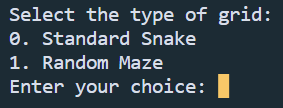
\includegraphics[scale=0.7]{Setup_1} 
    \caption{First setup screen allows switching between a standard grid and a random maze}
    \label{fig:subim1}
\end{subfigure}
\begin{subfigure}{0.3\textwidth}
    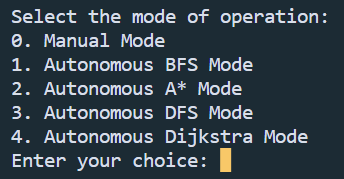
\includegraphics[scale=0.7]{Setup_2}
    \caption{Second setup screen allows user to choose moode of operation}
    \label{fig:subim2}
\end{subfigure}
\begin{subfigure}{0.3\textwidth}
    
\includegraphics[scale=0.7]{Maze_Generation}
    \caption{Maze setup screen allows user to decide on height and width of grid as well as density of maze}
    \label{fig:subim3}
\end{subfigure}

\caption{Setup screens in the program}
\label{fig:image1}
\end{figure}

\begin{figure}[H]
\centering
\begin{subfigure}{0.24\textwidth}
    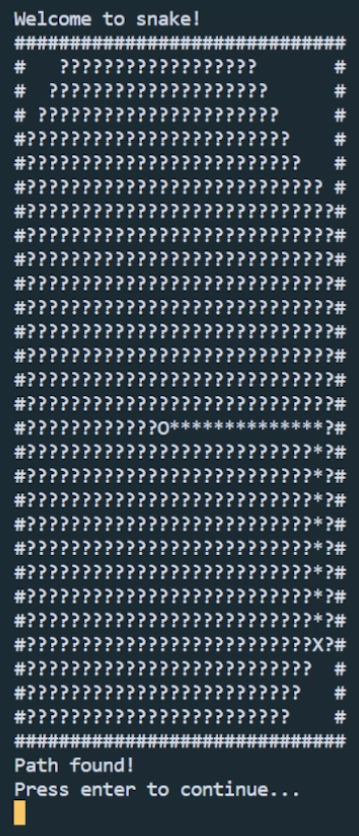
\includegraphics[height=6.5cm]{BFS_Path_found} 
    \caption{BFS}
    \label{fig:subim1}
\end{subfigure}
\begin{subfigure}{0.24\textwidth}
    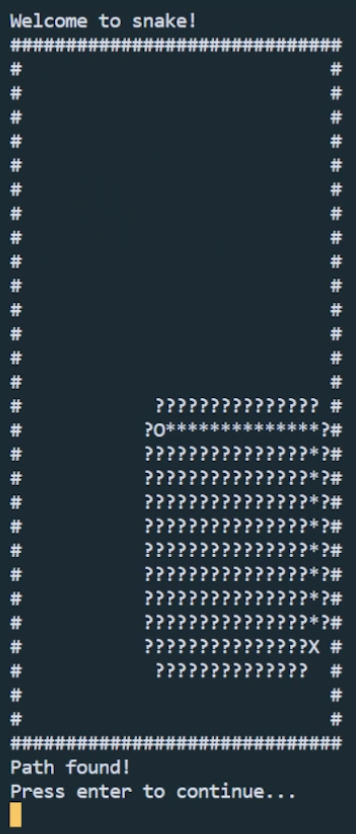
\includegraphics[height=6.5cm]{A_Star_Path_Found}
    \caption{A*}
    \label{fig:subim2}
\end{subfigure}
\begin{subfigure}{0.24\textwidth}
    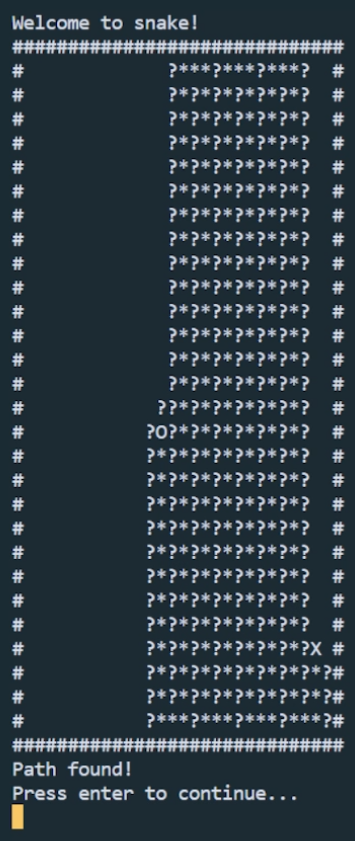
\includegraphics[height=6.5cm]{DFS_Path_Found}
    \caption{DFS}
    \label{fig:subim3}
\end{subfigure}
\begin{subfigure}{0.24\textwidth}
    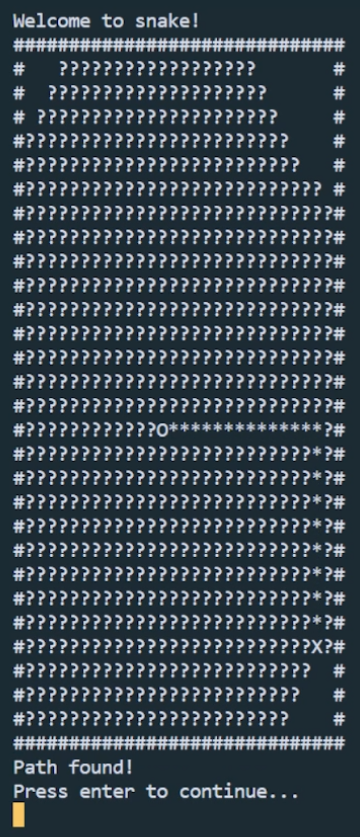
\includegraphics[height=6.5cm]{Dijkstra_Path_Found}
    \caption{Dijkstra}
    \label{fig:subim4}
\end{subfigure}

\caption{If autonomous mode is selected on a standard grid, the algorithm first performs a search using the specified algorithm. Dijkstra search is similar to BFS due to equal weights. 
The screen then displays the shortest path found (or any path in the case of DFS) and the snake moves in that direction. (?) is used to show visited cells and (*) is used to show the final path}
\label{fig:image2}
\end{figure}

\begin{figure}[H]
\centering
\begin{subfigure}{0.24\textwidth}
    
\includegraphics[height=6.5cm]{Maze_Generated} 
    \caption{Maze generated}
    \label{fig:subim1}
\end{subfigure}
\begin{subfigure}{0.24\textwidth}
    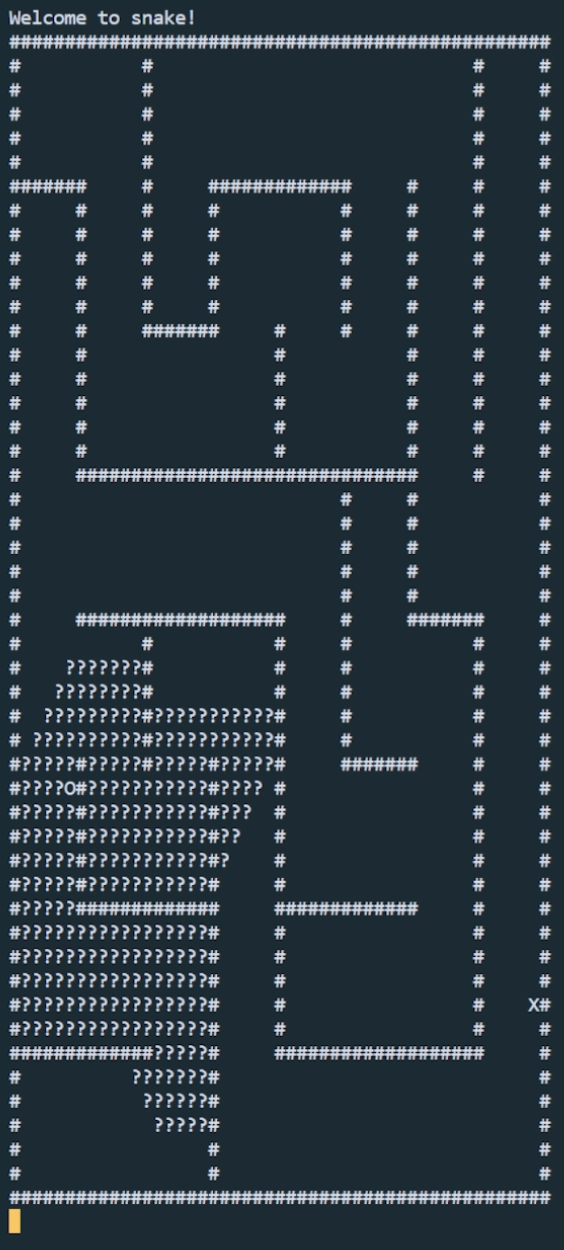
\includegraphics[height=6.5cm]{A_Star_Search_Maze}
    \caption{A* search}
    \label{fig:subim2}
\end{subfigure}
\begin{subfigure}{0.24\textwidth}
    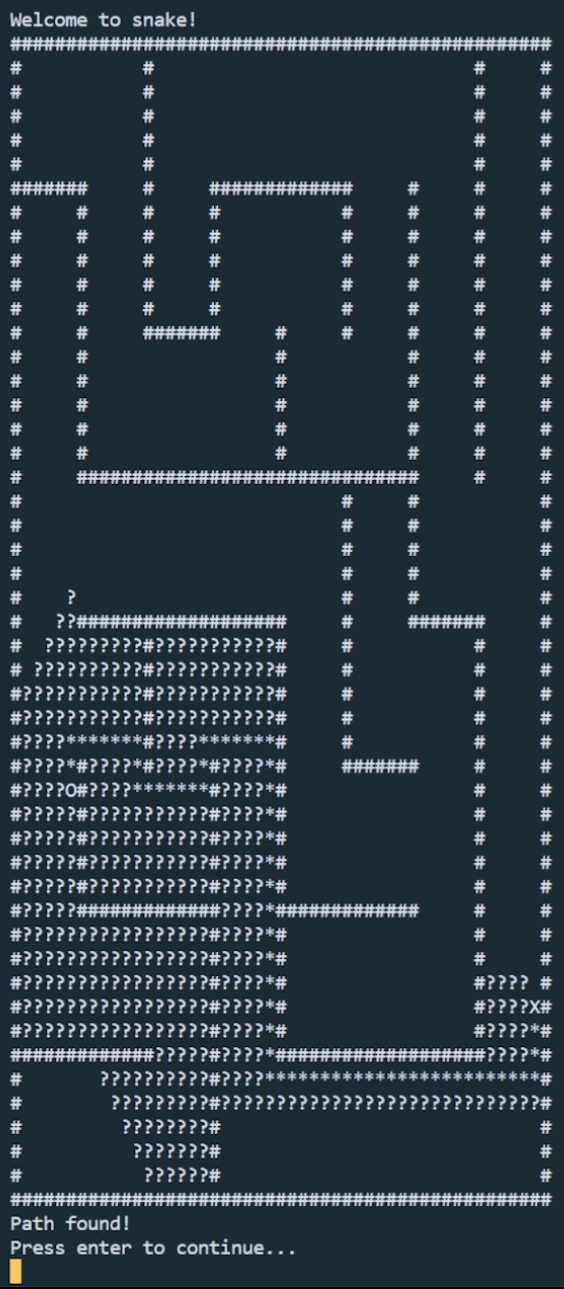
\includegraphics[height=6.5cm]{A_Star_Path_Found_Maze}
    \caption{A path is found}
    \label{fig:subim3}
\end{subfigure}
\begin{subfigure}{0.24\textwidth}
    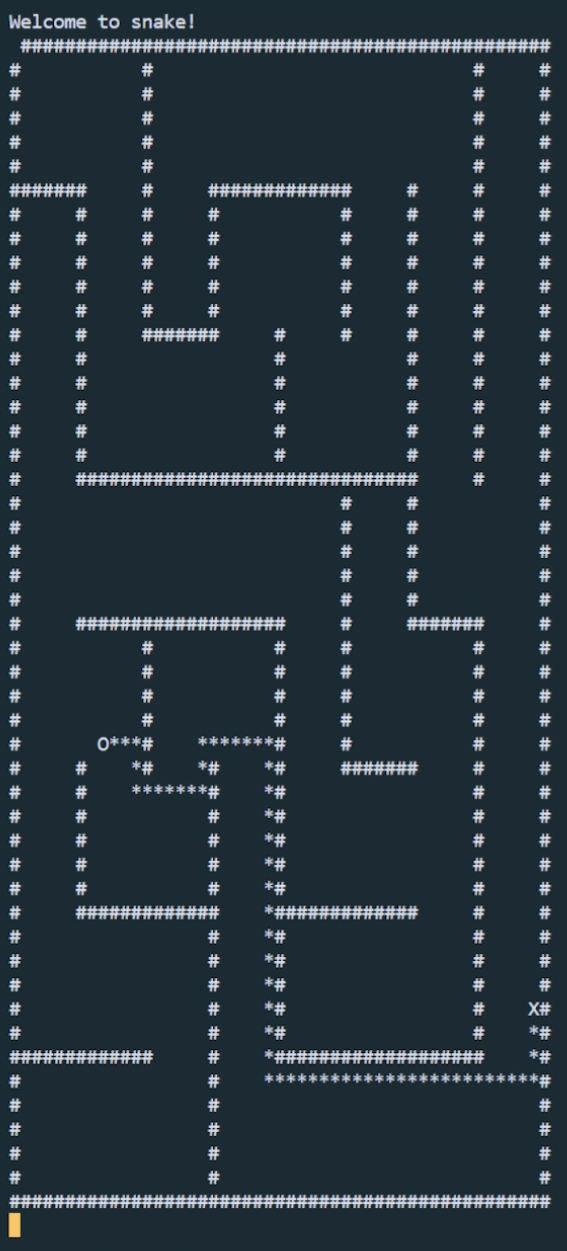
\includegraphics[height=6.5cm]{A_Star_Move_Maze}
    \caption{Snake moves}
    \label{fig:subim4}
\end{subfigure}

\caption{If the user selects a random maze, the process is very similar but a maze is first generated}
\label{fig:image3}
\end{figure}

\subsection{Design}

The extension is split up into the following files.
\begin{itemize}
    \item Main File: This provides setup functions, game logic and allows the user to interface with the game in manual mode.
    \item Maze: This uses a maze generation algorithm to generate a random maze. Demonstrates search algorithms in more difficult situations.
    \item Search Algorithm Files: These provides implementations for DFS, BFS, Dijkstra and A* algorithms.
    \item Game Utils: This provides game and input logic for players to interact with the game.
    \item Path Finding Utils: This provides common functions used by the search algorithms.
    \item Global: Global variables and structs used by multiple files.
\end{itemize}

\subsection{Problems}

\begin{itemize}
    \item Manual Mode: One problem was that the user needed to be able to control the snake without pressing the Enter key after each move. This would not be possible in a regular terminal 
    so we used the terminal in non canonical mode. This allowed us to read input as soon as it was available.
    \item Animation: We needed to animate the movements of the snake. We did this by clearing the terminal and redrawing the grid after each move. This could possibly be improved by using external libraries.
    \item Printing searches: One significant problem was printing the searches as they happened. While the search happened, this was not educational on its own as there was no 
    visualisation of the search. We experimented with having a separate grind to show the search as it happened but this was not very effective. We decided to pause the game every time the fruit is reached, 
    show the search happening and the shortest path found, then continue the search. This was a good compromise between showing the search and not interrupting the game too much.
    \item Maze Generation: We also found it difficult to integrate our maze generation algorithm with the game. We used print debugging to find the problem and fixed it.
    \item Memory Leaks: We also had memory leaks in our code which we fixed using Valgrind.
\end{itemize}

\subsection{Extension Testing}
As our project was a game which requires human interaction it was hard to test. We mainly tested by playing the game repeatedly and trying unusual sequences of inputs or actions such as reversing direction of the snake, 
touching corners, crashing into walls or the body of the snake etc. However, it is impossible for us to predict every possible sequence of actions a user might take. Therefore, our testing may not be very effective without 
a large number of users testing the game. However, since Snake is a fairly simple game, it is likely that our testing is sufficient.

\section{Group Reflection}

Since the start of the project we have had weekly group meetings in the library to discuss the project in
detail and split up the workload between the four of us. Between these meetings we have been letting eachother 
know exactly what part of the code we are about to work on in order to avoid situations where two people do the 
same work. Our communication has meant that we have always known what our next step is individually as well as 
being able to track our progress as a group and make sure we are progressing at a good pace.
For our future group projects, we learned that we should spend time figuring out which parts of the project can 
be completed at the same time as this allows for work to be split up more effectively.
In the future we hope to have the same high level of communication with our groups for group projects as it 
speeds up work dramatically.

\section{Individual Reflections}

\subsection{Dina Duong}

abcd

\subsection{Maciej Rytlewski}

Based on my experiences during this project, as well as, feedback from my peers, I believe that I fit into the group very well and I found it easy to integrate into 
the group and get on well with the other members. I really enjoyed participating in this project, having worked on a large part of the Emulator, Assembler and assisting with part 3 
of the project too. To my own surprise, over the span of this project, I turned out to be our main code debugger, having debugged and fixed majority of the errors that were causing test failures 
within the Emulator and Assembler, which I did not expect to be a strength of mine. Due to this, I greatly developed my skills in using GDB to debug code, which turned out to be 
extremely useful to find the source of the errors within the code, which without GDB would've been much more difficult. On the other hand, I found that I quite struggled with 
the implementation of our Symbol Table ADT which I needed one of the other members to have a look at and help me with in the end, as I found it difficult to debug this particular 
section of code. I also found it quite difficult to deal with memory leaks and freeing allocated memory, as I was not able to figure out which allocated memory blocks are not being freed and where.
\newline
As my first ever big group project, this project has taught me a lot about working as a group. It made me understand how important communication is between your group members, to make sure 
that you are not working on the same parts of the program and to parallelise our work effectively. This project has also massively developed my skill and ability in using Git as previously, I had 
very rarely used Git and it was only for individual projects. Whereas, throughout this project, I was able to learn how to create new branches, merge branches, switch to different branches, resolve merge 
conflicts and generally utilise Git as a more collaborative tool, allowing me to understand how powerful it really is. I believe that all of these skills that I have developed throughout this project 
will be really useful to me in the future both in more group projects and individual projects too.

\subsection{Kritik Pant}

I believe that I fit in well in the group and got along with everyone. I helped with the development of the Emulator, Assembler and the Extension by 
making design decisions and implementing code which others were able to use and build upon. While I initially thought that the Emulator would be fairly easy, 
I found some parts quite difficult such as branching and dealing with different access modes. I also found it difficult to solve memory issues, often relying on 
other members of the group to help me. This was especially true in the Assembler where I worked on the implementation of the Symbol Table. While I found it fairly 
simple to build a basic table using a linked list similar to Java, I found it difficult to diagnose and solve memory issues arising from my implementation. 
Unexpectedly, I found the Extension to be a strength of mine due to my familiarity with path-finding algorithms and the game of Snake. I ran into some difficult 
problems described above but, due to my knowledge of the Linux command line, I was able to solve them.
\newline
Through this project, I learnt the importance of maintaing good communication and coordination between group members. Since we always kept each other updated 
on progress and what we were working on, we were able to avoid duplication of work and it was easier for members to help each other. I aim to continue this in 
future projects. I also improved my ability to use Git. Previously, I had only used Git as a version tracking system on personal projects. However, this project 
really showed me the power of Git as a collaboration tool. I learnt how to use branches to experiment with code and how to use merge requests to review and merge code. 
I also learnt how to use Continuous Integration to speed up testing. I believe that these skills will be helpful in future projects and I aim to research more about 
the features of Git and Gitlab to improve my workflow.

\subsection{Matty Williams}

Early on in the development of our project I discovered that I did not know how to use git in a collaborative way as I had never needed to 
when working on individual projects. During the project I have learned how to create branches, pull and push changes properly and resolve merge conflicts which will 
make git a strength of mine as opposed to a weakness going into future projects.
\newline
Another weakness of mine that was pointed out by my group is the fact that I don't add many comments to my code which can make the code hard to follow for other people.
After receiving this feedback I made an effort to comment the purpose of every function or confusing block of code that I wrote to make it easier for others to spot errors
in and fix my code where necessary.
\newline
I feel that a strength of mine was the ability to problem solve as I was able to come up with a way to parse the input file into an array of tokenised lines which could then
be assembled into binary. I was also able to fix problems with the implementation of the pathfinding algorithms in the extension.   
\newline
As a group I believe that we worked very well and we all got along well with eachother. In future projects I would like to be just as communicative, however I would split the
workload up differently between group members to ensure every part of the project is prioritised equally.

\end{document}
